\subsection{Decorator}
Viene utilizzato per aggiungere funzionalità ad un oggetto dinamicamente, senza usare il subclassing.
Si vuole \textit{"wrappare”} un componente dentro un decoratore per aggiungergli delle funzionalità. Per rendere più potente il tutto, sfruttando un’interfaccia comune è possibile decorare un decoratore e così via.
Al livello implementativo il Component dovrebbe essere stateless e le modifiche apportate dal Decorator dovrebbero essere leggere, in altri casi conviene usare il pattern Strategy, in modo da evitare decoratori costosi da manutenere.

\begin{figure}[ht]
    \centering
    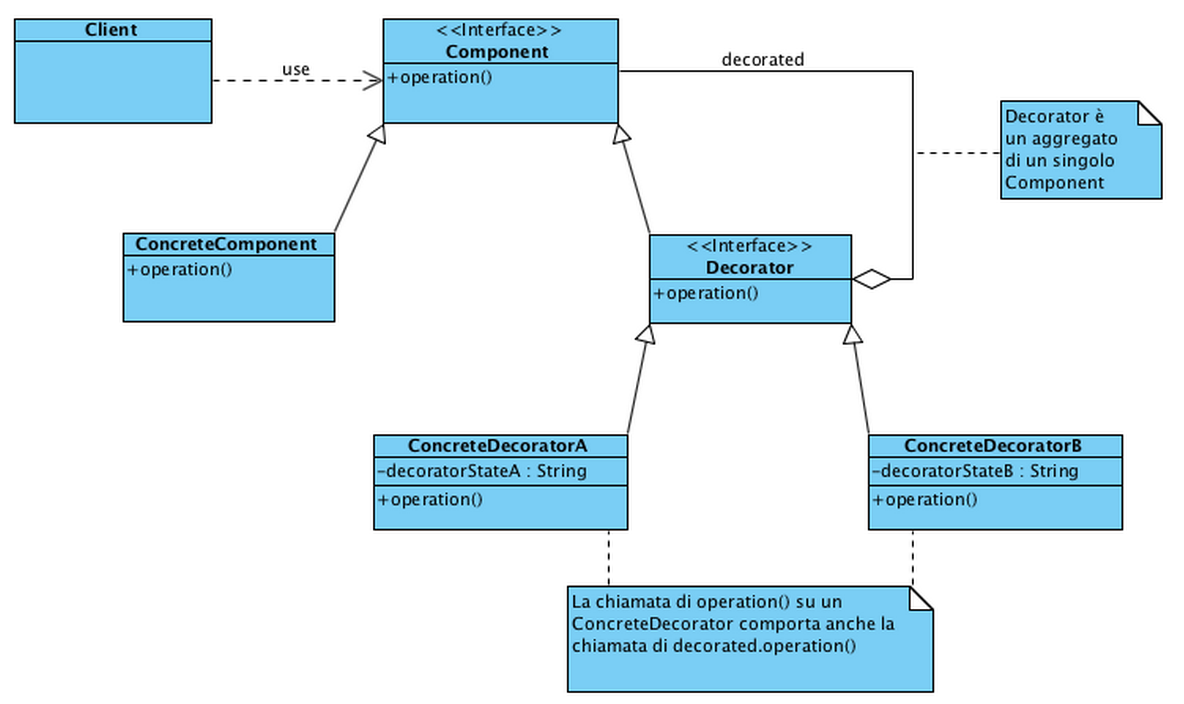
\includegraphics[width=0.8\textwidth]{immagini/decorator.png}
    \caption{Decorator}
\end{figure}
\FloatBarrier
\subsubsection{Utilizzo}
Prima creo il ConcreteComponent, poi usando creo i vari Decoratori, passandogli come riferimento il compoente: \\
\texttt{Component c = new ConcreteDecoratorB(new ConcreteDecoratorA(new ConcreteComponent));}
